\documentclass[a4paper, 14pt]{article}
\usepackage[T1]{fontenc}
\usepackage[utf8]{inputenc}
\usepackage[french]{babel}
\usepackage{subfiles}
\usepackage{ dsfont }
\usepackage{hyperref}
\usepackage{graphicx}
\usepackage{amsmath}
\usepackage{float} % Utilisation strict du positionnement des images
\author{Tuo Ismaël Maurice}
\date{14/04/2025}
\begin{document}
	\section{Définition}
	La similitude par cosinus permet de déterminer le degré de similitude entre deux phrases par calcul du cosinus de l'angle formé par les deux vecteurs de chacune de ces phrases.\\
	Soit les phrases suivantes:
	\begin{enumerate}
		\item Bonjour John.
		\item Bonjour Doé.
	\end{enumerate}
	On remarque que les deux phrases sont similaires mais comment le savoir avec un ordinateur.

	\section{Exemple Simple espace à 2 dimensions}
	Soit les phrases:
	\begin{enumerate}
		\item Bonjour John.
		\item Bonjour.
	\end{enumerate}
	On remarque qu'une des deux phrases est constituée  de deux mots donc on peut les représenter dans un espace à deux dimensions.\\
	On crée le tableau de similitude suivant:
	\begin{table}[H]
		\centering
		\begin{tabular}{|c|c|c|}
			\hline
			\textbf{Phrases} & \textbf{Bonjour} & \textbf{John} \\
			\hline
			Bonjour John & 1 & 1 \\
			Bonjour & 1 & 0 \\
			\hline
		\end{tabular}
		\caption{Tableau de similitude simple exemple 1}
		\label{tab:exemplesimple}
	\end{table}
	La représentation dans un repère donne:
	 \begin{figure}[H]
		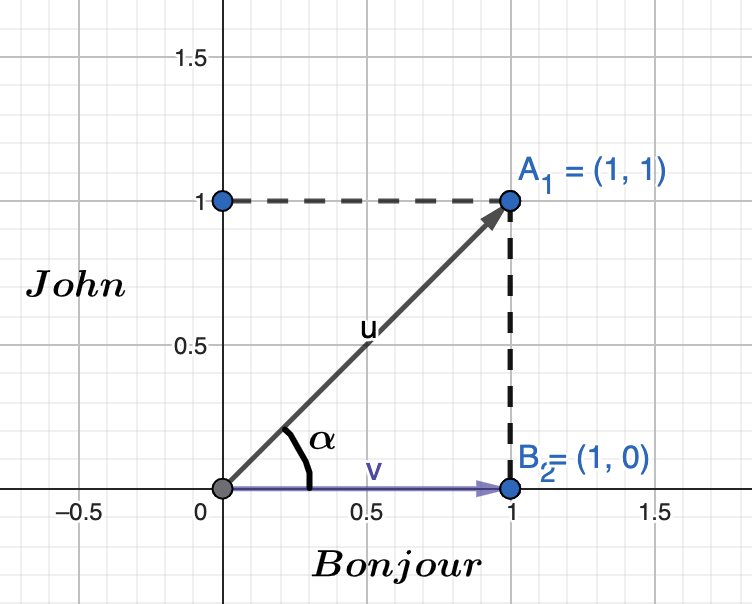
\includegraphics[scale=0.5, width=15cm]{./img/vecteur_exemple_simple.png}
		\caption{Représentation simple similitude exemple 1}
	\end{figure}
	La phrase 1 est représentée par le vecteur $A_{1}(1, 1)$ et la phrase 2 par le vecteur $B_{2}(1, 0)$.\\
	L'angle formé par ces deux vecteurs est l'angle $\alpha$ dont le cosinus permet de calculer la similarité entre les deux phrases.\\
	Dans l'exemple précédent, $\alpha=45^{o}$ dont $cos(\alpha)=0.71$. Soit $71\%$ de chance que les deux phrases soient similaires.\\
	Supposons que la phrase 2 soient \textbf{Bonjour, Bonjour, Bonjour.} alors on aura :
		\begin{table}[H]
		\centering
		\begin{tabular}{|c|c|c|}
			\hline
			\textbf{Phrases} & \textbf{Bonjour} & \textbf{John} \\
			\hline
			Bonjour John & 1 & 1 \\
			Bonjour, Bonjour, Bonjour  & 3 & 0 \\
			\hline
		\end{tabular}
		\caption{Tableau de similitude simple exemple 2}
		\label{tab:exemplesimple}
	\end{table}
	La représentation dans un repère donne:
	 \begin{figure}[H]
		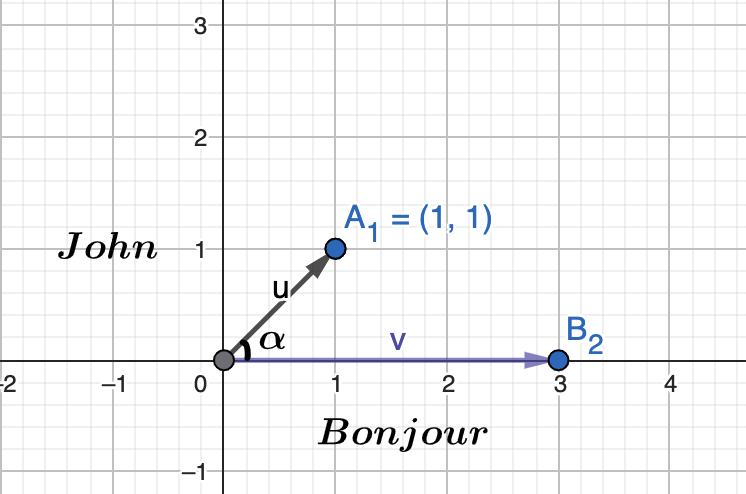
\includegraphics[scale=0.5, width=15cm]{./img/vecteur_exemple_simple_example2.png}
		\caption{Représentation simple similitude exemple 2}
	\end{figure}
	\textbf{Peut importe la longueur de  la phrase 2 le nombre d'ajout de \textit{Bonjour} ne change pas le $cosinus$ de $\alpha$.}
    \paragraph{Résumé:} La similitude par cosinus (\textit{cosine similarity en anglais}) est le cosinus de l'angle formé entre deux vecteurs et permet de révéler la similitude entre ceux-ci. Sa valeur est toujours entre 0 et 1.

    \section{Cas de similitude exacte}
    Soient les deux phrases suivantes:
    \begin{enumerate}
    	\item Bonjour John
    	\item Bonjour John
    \end{enumerate}
    On a comme comme tableau de similitude:
    \begin{table}[H]
    	\centering
    	\begin{tabular}{|c|c|c|}
    		\hline
    		\textbf{Phrases} & \textbf{Bonjour} & \textbf{John} \\
    		\hline
    		Bonjour John & 1 & 1 \\
    		Bonjour John  & 1 & 1 \\
    		\hline
    	\end{tabular}
    	\caption{Tableau de similitude exacte}
    	\label{tab:similariteexacte}
    \end{table}
    \newpage
    La représentation dans un repère donne:
    \begin{figure}[H]
    	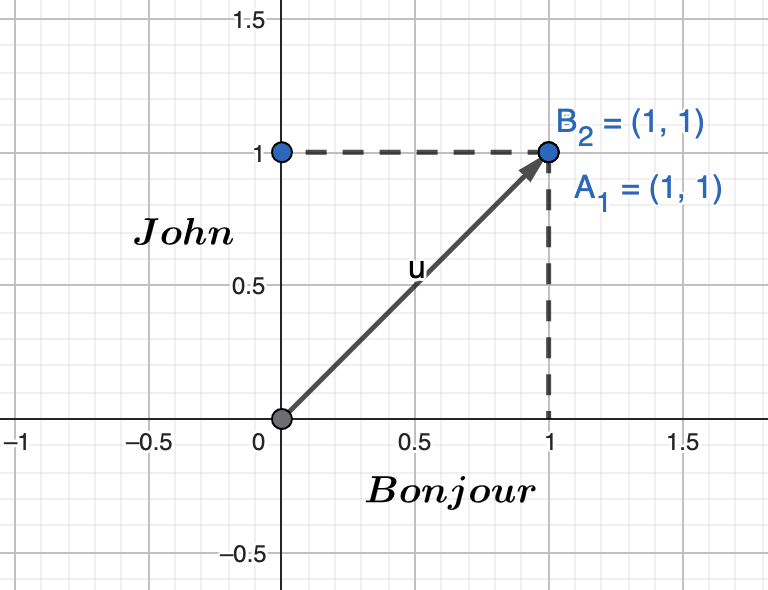
\includegraphics[scale=0.5, width=15cm]{./img/vecteur_similitude_exacte.png}
    	\caption{Représentation similitude exacte}
    \end{figure}
    Les deux vecteurs sont confondus donc $\alpha = 0^{o}$ soit $cos(\alpha)=1$ soit 100\% de chance que les deux vecteurs soient similaires. On peut conclure que les deux phrases sont totalement similaires.

    \section{Cas d'aucune similitude}
    Soient les deux phrases suivantes:
    \begin{enumerate}
    	\item Bonjour.
    	\item John.
    \end{enumerate}
	Le tableau de similitude donne:
	  \begin{table}[H]
		\centering
		\begin{tabular}{|c|c|c|}
			\hline
			\textbf{Phrases} & \textbf{Bonjour} & \textbf{John} \\
			\hline
			Bonjour & 1 & 0 \\
			John  & 0 & 1 \\
			\hline
		\end{tabular}
		\caption{Tableau de non similitude}
		\label{tab:nonsimilarite}
	\end{table}
	\newpage
	La représentation dans un repère donne:
	\begin{figure}[H]
		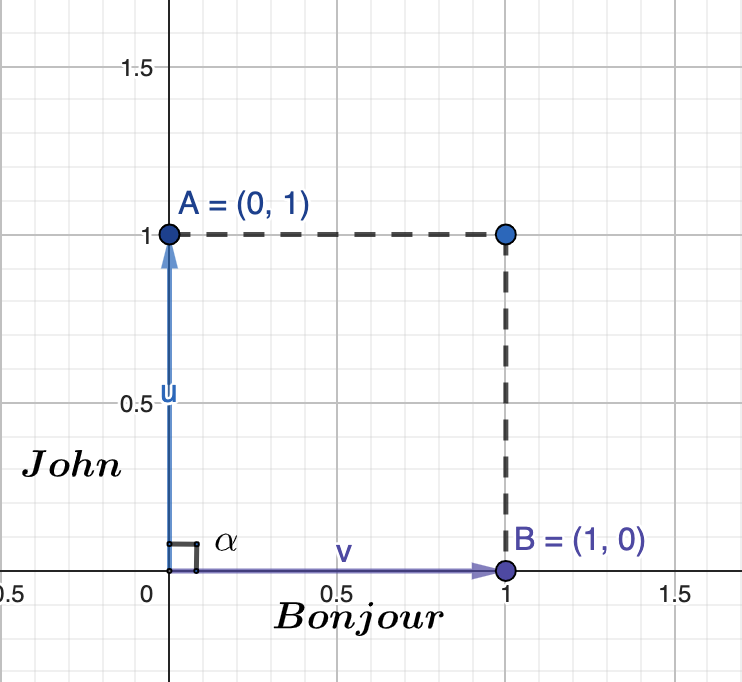
\includegraphics[scale=0.5, width=15cm]{./img/vecteur_non_similitude.png}
		\caption{Représentation non similitude}
	\end{figure}
	L'angle formé par les deux vecteurs est $\alpha = 90^{o}$ donc $cos(\alpha) = 0$ soit 0\% de chance que les deux vecteurs soient similaires. On peut conclure que les deux phrases sont totalement différentes.

    \section{Résumé}
	  \[
	  cos(\alpha) =
	  \begin{cases}
	  	0&\text{Si aucune similitude entre les deux phrases.}\\
	  	1 & \text{Similitude totalement exacte.}\\
	  	\in ]0, 1[ & \text{Sensiblement similaires quand les deux phrases ont en commun des mots.}
 	  \end{cases}
	  \]
		Pour avoir le \textbf{cosinus} de la similitude entre deux phrases suivre les étapes suivantes:
		\begin{enumerate}
			\item Faire un tableau de fréquence des mots (compter le nombre d'occurrences de chaque mot dans chacune des phrases).
			\item  Afficher les points.
			\item Trouver l'angle entre Vecteurs.
			\item Calculer le cosinus de l'angle formé.
		\end{enumerate}

    \section{Cas complexes}
    Les cas précédents marchent pour des phrases avec deux mots c'est à dire représentables dans un espace à 2 dimensions $\mathds{R} \text{x} \mathds{R}$. \\
    Les phrases de la vie réelle sont de plusieurs mots soit représentables dans un espace $\mathds{R}^{n}$, dans ce cas on utilise la formule suivante:
   	\[
   		cos(\alpha) = \frac{\sum_{i=1}^{n}A_{i}B{i}}{\sqrt{\sum_{i=1}^{n}A_{i}^{2}} * \sqrt{\sum_{i=1}^{n}B_{i}^{2}}}, avec \ i = \  \text{indice des mots}
   	\]
   	Soient les phrases suivantes:
   	\begin{enumerate}
   		\item Bonjour John
   		\item Bonjour
   	\end{enumerate}
   	 \begin{table}[H]
   		\centering
   		\begin{tabular}{|c|c|c|}
   			\hline
   			\textbf{Phrases} & \textbf{Bonjour} & \textbf{John} \\
   			\hline
   			Bonjour John & 1 & 1 \\
   			Bonjour  & 1 & 0 \\
   			\hline
   		\end{tabular}
   		\caption{Tableau de similitude avec formule}
   		\label{tab:similitude}
   	\end{table}
   	Le calcul de la similitude donne:
   	\[
   		cos(\alpha) = \frac{(1*1) + (1*0)}{\sqrt{1^{2} + 1^{2}} * \sqrt{1^{2} + 0^{2}}} = \frac{1}{\sqrt{2} * 1} = 0.7071
   	\]
   	Soit les $cos(45)$ trouvé précédemment.\\
   	Soient deux phrases:
  	\begin{enumerate}
  		\item Bonjour tout le monde.
  		\item Bonjour John
  	\end{enumerate}
  	Le tableau de similitude donne:
  	\begin{table}[H]
  		\centering
  		\begin{tabular}{|c|c|c|c|c|c|}
  			\hline
  			\textbf{Phrases} & \textbf{Bonjour} & \textbf{tout} & \textbf{le} & \textbf{monde} & \textbf{John}\\
  			\hline
  			Bonjour tout le monde. & 1 & 1 & 1 & 1 & 0 \\
  			Bonjour  John & 1 & 0 & 0 & 0 & 1 \\
  			\hline
  		\end{tabular}
  		\caption{Tableau de similitude plusieurs dimensions}
  		\label{tab:similitudecomplexe}
  	\end{table}
	Le calcul de la similitude donne:
	\[
		cos(\alpha) = \frac{(1*1) + (1*0) + (1*0) + (1*0) + (0*1)}{\sqrt{1^{2} + 1^{2} +  1^{2} +  1^{2} + 0^{2}} * \sqrt{1^{2} + 0^{2} + 0^{2} + 0^{2} + 1^{2}}} = \frac{1}{2 * \sqrt{2}} = 0.35
	\]
	Soit 35\% de chance d'être similaires.

    \section{Aller plus loin}
    Le soucis avec cette méthode est que la similitude se base sur la construction des mots (plan syntaxique/grammatical) donc deux mots \textbf{Bonjour} et \textbf{Hello} seront considérés comme non similaires car le sens implicite n'est pas pris en compte.\\
    De même \textbf{Beau} et \textbf{Belle} seront considérés comme non similaires.\\
    Dans les projets, on utilisera le lemme des mots c'est à dire la forme de base du mot. Avec l'utilisation du lemme on aura:
    \begin{enumerate}
    	\item[\textbullet] beau => lemme beau
    	\item[\textbullet] belle => lemme beau
    \end{enumerate}
    En utilisant les lemmes \textbf{Beau} et \textbf{Belle} seront représentés par leur forme lemmatisée et donc similaire.\\
    De plus, cette méthode ne prend pas en compte le sens sémantique entre deux phrases c'est à dire deux phrases \textbf{Le chat mange la souris} et \textbf{La souris mange le chat} seront considérées comme similaires au plan syntaxique et grammatical mais sur le plan sémantique (du sens) elles sont totalement différentes.\\
    Pour aller plus loin sur le sujet, on peut utiliser les librairies de NLP (Natural Language Processing) comme \href{https://spacy.io/}{SpaCy} et \href{https://www.nltk.org/}{NLTK} qui contiennent des outils de traitement automatique des langues.
\end{document}